Differences in gender are well-known facts of economic and social life. This paper investigates how participation in enriched early childhood programs differentually enhances the lives of disadvantaged boys and girls, and whether they enhance or reduce gender gaps among the disadvantaged children.

There is a rich literature in psychology on the greater vulnerability of boys to adverse life conditions.\footnote{See \cite{Schore_2017_IMHJ} for an extensive survey. Economists have contributed to this literature. See, e.g., \cite{Autor-etal_2015_Family-Disadvantage}.} As a group, girls mature earlier, are more resilient to adversity, and perform better on a variety of lifetime measures. Less is known about effective strategies for reducing the vulnerability of boys to disadvantaged childhoods. This paper uses data from an influential, widely emulated, early childhood program to investigate these issues.

Specifically, we analyze data from a randomized controlled trial of a prototypical intensive early childhood program that enriched the early lives of disadvantaged children. The program is widely emulated and is a template for many current and proposed early interventions. The program starts at eight weeks of age and continues through age 5. Participants and controls are followed through age 34 with data collected at all stages of the life cycle.

We study the differential impact of the program by gender on a variety of life outcomes. There are positive impacts of the program for both genders, but there are also important substantial differences in impact by gender across the life cycle. We also study the impact of home care versus low quality center care on control group children by gender. Boys placed in low quality center environments do much worse than girls. This is consistent with a large body of work in psychology on the importance of early attachment on the lives of boys. Boys benefit more from high quality center care than girls, although both genders benefit.


The program we analyze, the Carolina Abecedarian Project (ABC) and its sister program, Carolina Approach to Responsive Education (CARE), were conducted in Chapel Hill, North Carolina for a sample of children born between 1972 and 1980. We refer to the combined programs as ABC/CARE.

As a preview of our analysis, we report gender differences of outcomes in Figure~\ref{fig:intro-skills-plots-skills}. Females perform, on average, about five quantiles better than males on early measures of social-emotional skills.\footnote{This is consistent with previous work showing that females tend to outperform males on tests of skills \citep{Baker-Milligan_2013_Boy-Girl-Differences}.} There is a similar gender difference in the early measures of parenting, specifically the absence of punishment. Males receive more parental discipline than their female counterparts. Stark gender differences are not found for IQ or achievement measures.

The gender differences for income and education in the adult years are not significantly different. Males have slightly higher levels of both. Health, represented by adult BMI, is worse for females by about five quantiles. The opposite is true for crime.\footnote{Crime costs are estimated in \citet{Garcia_Heckman_Leaf_etal_2017_Comp_CBA_Unpublished}.}

\begin{figure}[!htbp]
\textbf{[JJH: Why these measures?]}
\centering
\caption{Differences Between ABC/CARE Males and Females}
\label{fig:intro-gdiff-plots}
\begin{subfigure}[h]{0.55\textwidth}
	\centering
	\caption{Skill Measurements}
	\label{fig:intro-skills-plots-skills}
	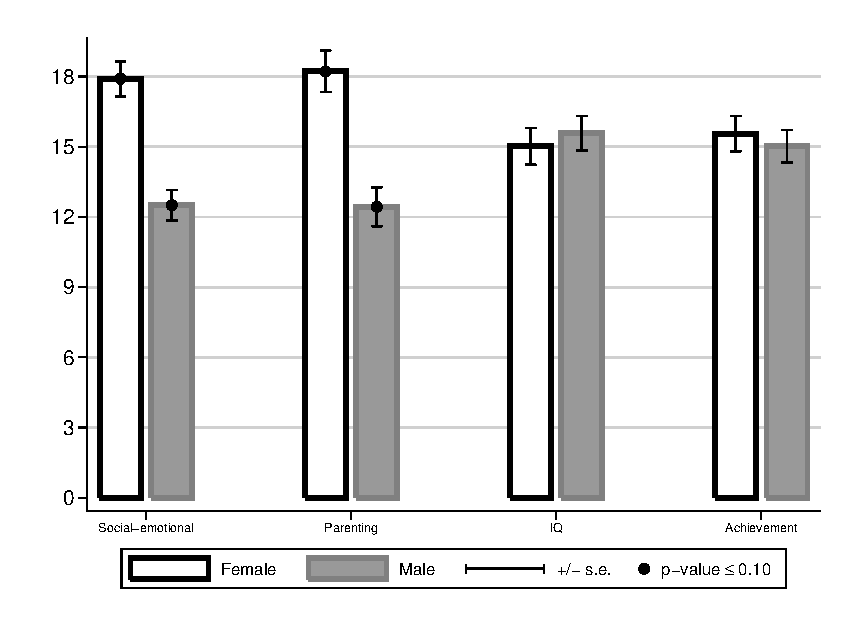
\includegraphics[width=\textwidth]{output/abccare-gdiff-skills}
\end{subfigure}

\begin{subfigure}[h]{0.55\textwidth}
	\centering
	\caption{Adult Outcomes}
	\label{fig:intro-skills-plots-adultsimp}
	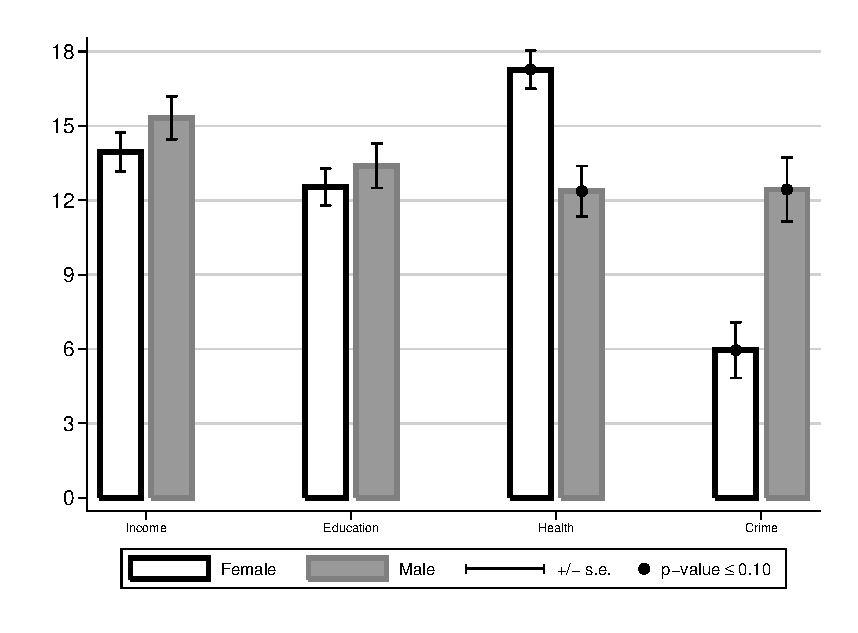
\includegraphics[width=\textwidth]{output/abccare-gdiff-adultsimp}
\end{subfigure}
\footnotesize \justify
Note: These plots show the means of select variables by gender, pooling across experimental groups. The capped lines show the standard errors and black points indicate that the female is significantly different than the males. These hypothesis tests are two-sided and computed using 100 bootstraps. All factor variables are calculated by principal factor analysis. The factors are then standardized and divided into 30 quantiles. Panel (a) Social-emotional is a factor of task-orientation measured by the Infant Behavioral Record (IBR; \citet{Bayley_1969_BSID-Manual}) at ages 0.5, 1, 1.5 years. Parenting is a factor of the absence of punishment scale of Home Observation for Measurement of the Environment (HOME; \citet{Elardo_Bradley_1981_DR}) between ages 0.5 and 4.5 years. IQ is a factor of full IQ scores measured by the Stanford-Binet Intelligence Scale (SB; \citet{Terman_Merrill_1960_BOOKSBintelligence}), McCarthy Scales of Children's Abilities (MC; \citet{McCarthy_1972_Manual-McCarthy-Scales}), and the Wechsler Preschool and Primary Scale of Intelligence (WPPSI; \citet{Wechsler_1974_Manual-WISC-R}) at ages 2, 3, 4, and 5 years. Achievement is a factor of reading and math scores measured by between the ages of 6 and 12 years. Panel (b) Income is the lifetime net present value of income predicted in \citet{Garcia_Heckman_Leaf_etal_2017_Comp_CBA_Unpublished}. Education is an indicator of high school graduation by 21 years. Heath is BMI measured at approximately 35 years. Crime is the net present value of projected crime costs as estimated in \citet{Garcia_Heckman_Leaf_etal_2017_Comp_CBA_Unpublished}. All of these adult variables are standardized and split into quantiles to be consistent with the skills.
\end{figure}

Although these mean differences do not include the effect of early childhood education on improving these skills, many studies have shown the potential for early-life interventions to improve the skills of children, especially those from disadvantaged families.\footnote{\citet{Currie_2011_AER,Elango_Hojman_etal_2016_Early-Edu}.} Several of these studies separate analysis by gender and find that males and females benefit differently from early childhood education. For example, \citet{Heckman_Moon_etal_2010_QE} and \citet{Garcia_Heckman_Leaf_etal_2017_Comp_CBA_Unpublished}, analyze randomized control trials with long-term data follow-ups, find that intervening early in life more positively affects education for females and labor market and health outcomes for males. Other studies analyzing programs with shorter-term data also find gender differences in early skills and academic outcomes.\footnote{\citet{Deming_2009_AEJAE,Ou_Reynolds_2010_Mechanisms_CYSR,Magnuson_Kelchen_Duncan_etal_2016_ECRQ}.}

This paper studies the treatment effects of ABC/CARE by gender. We report standard treatment effects comparing the treatment and control group. This considers the treatment effect given that the control-group families select the ``next best'' early childhood option for their children. This option can include staying at home or attending other center-based care.\footnote{Historical documentation, records, and evidence from knowledgeable individuals indicate that although these alternate centers followed state and federal standards, they were of lower quality than the ABC/CARE intervention.}

Unlike previous studies analyzing ABC/CARE, we additionally compute treatment effects comparing the treatment group to the control group fixing those in the control group to these two alternate counterfactuals.\footnote{Previous studies presenting treatment effects of ABC and CARE include \citet{Ramey_etal_1985_Project-CARE_TiECSE, Clarke_Campbell_1998_ABC_Comparison_ECRQ,Campbell_Pungello_etal_2001_DP,Campbell_Ramey_etal_2002_ADS,Campbell_Wasik_etal_2008_ECRQ,Campbell_Conti_etal_2014_EarlyChildhoodInvestments}.}$^,$\footnote{See \cite{Heckman_1992_randomization}, \cite{Heckman_Hohmann_etal_2000_QJE}, and \cite{Kline_Walters_2016_QJE} for work related to control substitution.}

Given the large number of available variables from the numerous follow-ups, summarizing all treatment effects can overwhelm the reader.\footnote{We consider a total of 95 outcomes that we classify in Appendix~\ref{appendix:results} \textbf{[JJH: These should go in text.]}.} In a companion paper, \citet{Garcia_Heckman_Leaf_etal_2017_Comp_CBA_Unpublished} aggregate the treatment effects by conducting a cost/benefit analysis. They show that the benefits from ABC/CARE are largely driven by its effects on males. The benefit/cost ratio is 10.19 for males and 2.61 for females. In this paper, we report treatment effects by category and the proportion of statistically significant effects. We use combining functions, which count the number of positive (and significant) treatment effects by gender. They indicate that females benefit more from the program than do males.

We find strong effects on education and employment for females with high school graduation increasing between 13 and 25 percent and employment increasing between 8 and 13 percentage points.\footnote{The range arrises from the different estimates.} Although the treatment did not increase education for males as strongly as for females, it increased employment between 11 to 19 percentage points and labor income between 19 and 24 thousand of 2014 US dollars.\footnote{Income, employment, and education were measured when the subjects were 30 years.}

We broaden the discussion of results to the full set of outcomes by presenting the estimates of the counts of positive treatment effects. To perform inference on these estimates, we test the hypothesis of whether the proportions are equal to 50\%. As Figure~\ref{fig:intro-cfunctions} shows, although the proportions for both genders are significantly greater than 50\%, the proportion is higher for females. When considering the proportion of outcomes that are both positive and significant at the 10\% level, we test the hypothesis whether the proportions are equal to 10\%.\footnote{Our inference accounts for the dependence across outcomes, as we explain in Section~\ref{sec:combining-functions}.} A similar pattern holds for this test as well, although the proportions are smaller. Across outcomes, the effects are stronger for males fixing the control group to alternate preschool, but stronger for females when fixing the control group to staying at home. This pattern holds in the individual treatment effects, the combining functions, and the results from \citet{Garcia_Heckman_Leaf_etal_2017_Comp_CBA_Unpublished}.

\begin{figure}[!htbp]
\centering
\caption{Proportion of Outcomes that are Positively Impacted}
\label{fig:intro-cfunctions}
	\begin{subfigure}[h]{0.7\textwidth}
		\centering
		\caption{Treatment vs. Next Best} \label{fig:ppositivenb}
		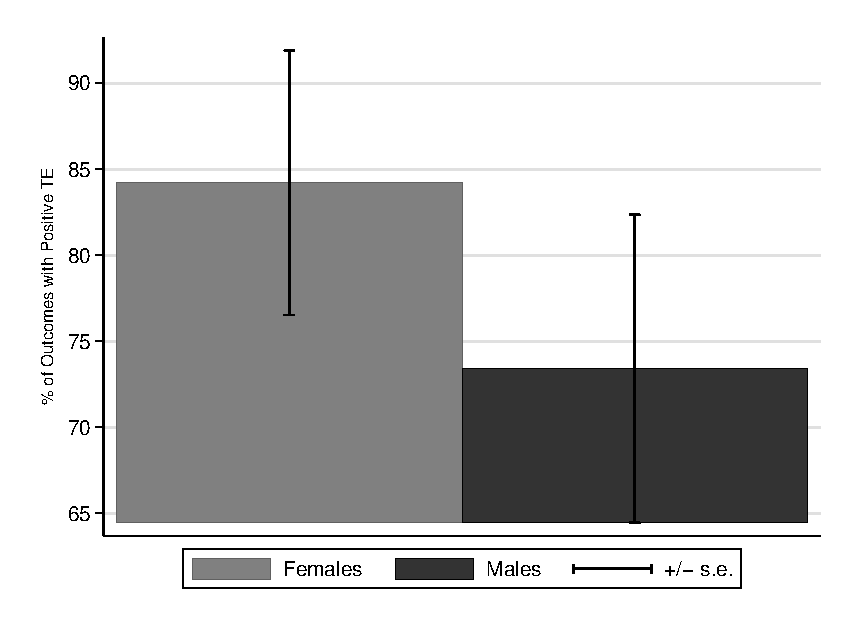
\includegraphics[width=\textwidth]{output/itt_noctrl_all.eps}
\end{subfigure}

\begin{subfigure}[h]{0.7\textwidth}
	\centering
	\caption{Treatment vs. Next Best, Significant at 10\% Level} \label{fig:ppositive10}
		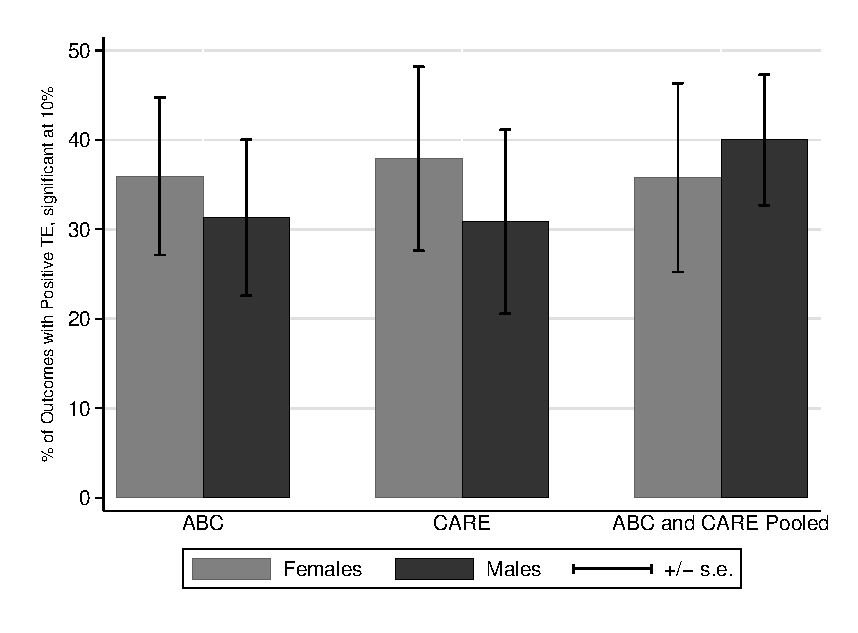
\includegraphics[width=\textwidth]{output/itt_noctrl_all_sig10.eps}
\end{subfigure}
\footnotesize \justify
Note: Panel (a) percentage of outcomes displaying a positive treatment effect, comparing treatment to next best. Panel (b) percentage of outcomes displaying a positive and statistically significant treatment effect (10\% significance level).
\end{figure}

\textbf{[JJH: Comes too early -- summarize and report later.]}

This difference in the results depending on the counterfactual, as well as the gender differences in the treatment effects, drives our discussion of the interaction between the treatment, the family inputs, and any potential alternate center-based care. The explanation that males are more fragile than females early in life is consistent with the early differences favoring females.\footnote{\citet{Kottelenberg-Lehrer_2014_Gender-Effects,Baker_Gruber_Milligan_2015_Noncog_Defects, Schore_2017_IMHJ}.} Building on this, we explore how these early-life differences evolve for specific outcomes that are central to the analysis of  \citet{Garcia_Heckman_Leaf_etal_2017_Comp_CBA_Unpublished}, such as crime and income. We find that the treatment compensates for males' early-life deficits, allowing the gaps between males and females to close for important adult outcomes.

The paper proceeds as follows. We describe ABC/CARE in more detail in Section~\ref{sec:data}. We then discuss the parameters of interest in Section~\ref{sec:parameters} and describe our method for summarizing over the multitude of variables in Section~\ref{sec:combining-functions}. Section~\ref{sec:treatment-effects} displays the estimates of the parameters of interest and the combining functions. We discuss suggestive mechanisms through which the early-life skill differences mediate later-life gender differences in Section~\ref{sec:gender-differences}. Section~\ref{sec:conclusion} concludes.


\textbf{[JJH: We need to report}
\begin{enumerate}[7(a)]
\item \textbf{Value added compared to home by gender (do we have results moderated by family background and by presence/absence of father?)}
\item \textbf{Comparison of control children---are girls doing better or worse?/also report moderators]}
\end{enumerate}


%ee \citet{Beeghly-etal_2017_IMHJ,Dayton_2017_IMHJ,Iruka_2017_IMHJ,Schore_2017_IMHJ} for recent findings on the topic of different development of males and females early in life. 